\begin{quote}
	\textit{``The major challenge for the future will be effectively and cheaply to shift the sense of presence from one's own body to another, without replacing or excluding the physical world in which we all exist.''}
\end{quote}
\hfill \textit{Distributed Embodiment: Real Presence in Virtual Bodies, Waterworth \& Waterworth}
\\
\\
%=========================================================================================================
%=========================================================================================================

\label{introduction}

%=========================================================================================================

A tourist steps into a 15th century chapel. Although the chapel is in remarkable condition for a building that is over 500 years old (it is even still in active use!) it looks markedly different today than it did when it was first built, back in 1450. The tourist dons a head-mounted display, which via a pair of front mounted cameras allows her to still see where she is going as she starts to walk through the chapel. Once in the centre of the chapel, she stops walking \& presses a button on a controller in her hand. Her view of the chapel around her disappears \& is replaced with a virtual reconstruction of the chapel as it stood over 500 years ago. The view changes appropriately as she turns her head, allowing her to look all around her at how chapel used to be.

She releases the button \& is returned to the present day \& continues walking through the chapel until she reaches the altar. She presses the button again \& once again her view switches to that of the virtual chapel, which has moved to match her new position at the altar, allowing her to inspect its 1450 counterpart.

This is not an augmented reality system, which superimposes virtual objects upon the real world. This is a \textbf{parallel reality} system that allows its user to switch between viewing the real world \& viewing a complete, immersive virtual environment that far exceeds the level of virtuality capable of being displayed by augmented reality.

%maybe participant-f-3.jpg here instead
%\begin{figure}[h]
%	\begin{center}
%		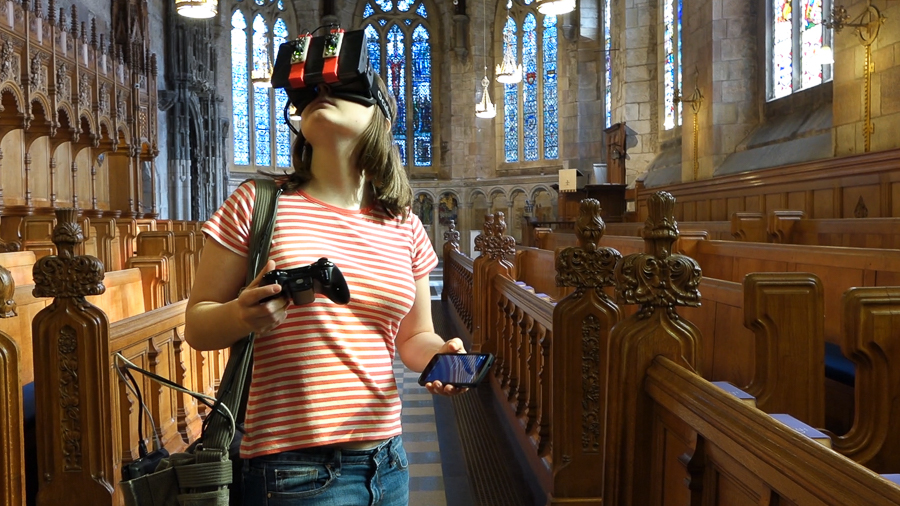
\includegraphics[width=\textwidth]{participant-f-2.jpg}
%		\caption[foo]{The \textit{Mirrorshades} parallel reality platform in use at a 15th century chapel.\footnotemark}
%		\label{participant-f-2.jpg}
%	\end{center}	
%\end{figure}

\afterpage{
\begin{figure}[h]
	\begin{center}
	   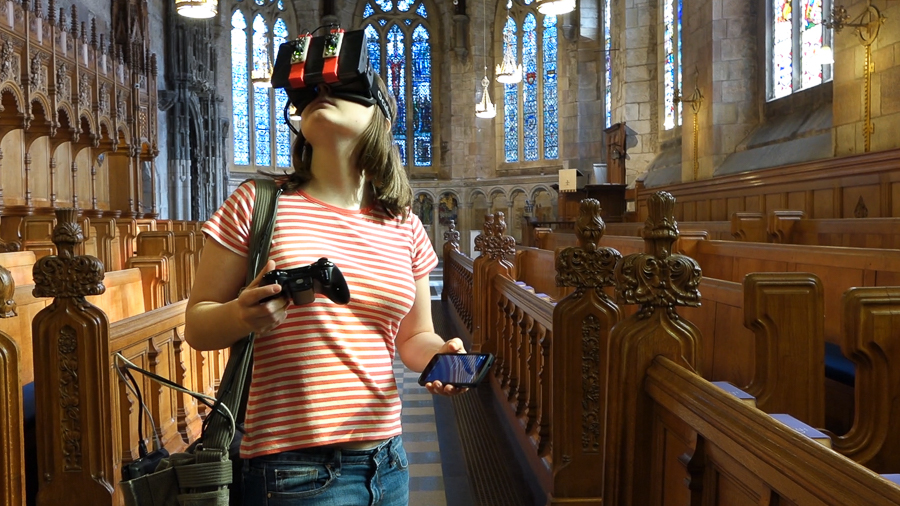
\includegraphics[width=\textwidth]{participant-f-2.jpg}
	\end{center}
	\label{participant-f-2.jpg}
	\caption{The \textit{Mirrorshades} parallel reality platform in use at a 15th century chapel. This image is taken from a video that is available to view online\protect\footnotemark\ .}
\end{figure}

\footnotetext{\url{https://www.youtube.com/watch?v=UsDRPjDwr8A}}
}

%=========================================================================================================

\section{Parallel Reality}

The central theme of this thesis is the concept of `parallel reality', defined thus;

\textbf{Parallel Reality:} A system comprising two environments, one real \& the other virtual with each complete unto itself, wherein the user is granted the ability to freely transition between receiving stimuli from either.
 
%=========================================================================================================

\section{Contributions}

%=========================================================================================================

\section{Research Domains}

%=========================================================================================================

\section{Document Overview}

%=========================================================================================================

















%=========================================================================================================



Talk about history of alternate realities, talk about the disappointment of VR in the 90's \& it's resurgence now thank to Oculus, etc.






Alternate realities have been a mainstay of both popular science fiction \& of serious academic research, the concept of the existence of another `there' \& how we could visit it or bring it into our `here'
keeping authors \& scientists alike fascinated for many decades.

From the `Sensorama' simulator of the 1960s to the Oculus Rift of the early 2010s

From William Gibson's `The Gernsback Continuum' \& beyond through contemporary cyberpunk literature

the `gargoyles' of MIT


The 90's saw a surge of hype over the Virtual Reality concept, however with hardware \& software not ready to meet the expectations sown among consumers by the media the bubble burst.

The advent of the smartphone lead to the dissemination of any number of Augmented Reality, an attempt to merge to some extent our real world with aspects of the virtual.


And the Media Lab invented what they would call Cross Reality that linked a real world location with a virtual other via sensors \& actuators, such that an inhabitant of one could glimpse a tantalizing insight into the goings on of the `other' although they could not see into it.

This thesis explores an alternate reality that as yet has received little attention or even a name. Parallel Reality as it came to be called builds upon the concept of Cross Reality \& its two distinct environments each `complete unto itself'. But instead of the shadow of one environment only laying upon the other by manner of sensors \& actuators, new VR technology combined with indoor positioning systems allow a user to switch between environments - to at one moment view their RW surroundings \& at the next to view the equivalent vantage in a parallel virtual environment

%=====================
%On why alternate realities are predominantly visual?

\textit{``visual ordination of intellectual knowledge''}

\textit{``Seeing remains an insistent metaphor for all of cognition only because while the ocular lobes are merely one of our brain's tentacular connections to reality, they are among the most `conscious' of their capacity for information control.''}

The Mediated Sensorium, Caroline A. Jones



Caroline A. James speaking on the work of Janet Cardiff \& George Bures Miller

\textit{``Cardiff brings segmentation into the present, crafting `sound walks' that layer an alternate reality over the fl\^aneur's perambulations - a fantastic elaboration of the kind of personal soundscape chosen by the iPod user.''}


\textit{``Sight plays such a prominent part in the mental life that the field of vision is sometimes considered almost synonymous with the field of attention.''}~\cite{Lucas1951}

%=========================================================================================================

Structure of thesis here